\section{Methods}
\label{sec:Methods}

\subsection{Manufacturing}

\subsubsection{Preparation of Chemicals}

All chemicals were of analytic grade and were used as received from the suppliers without further  purification. Every chemical was bought from Sigma Aldrich, unless stated otherwise. 
Next for facilitation we introduced the formula making use of stoichiometry:

\begin{equation}
\label{eq:RedPrep}
    \frac{m'\cdot v\cdot M}{1000} = m(m',v,M)
\end{equation}


where $m'$ denotes the molecular weight of the reagent, $v$ the desired end-volume of the solution, $M$ the molar concentration and $m$ the needed amount of the substance with unit 'grams', assuming the chemical to be pure. (Example: We want to make 4ml (~$= v$) of solution with \ce{NaOAc} (~$m'_{\ce{NaOAc}}= 82.03 \frac{g}{mol}$) at a concentration of 0.25 M (~$= M$). We now know, that we need to dilute $m \approx 82mg$ \ce{NaOAc} in 4ml of solvent!) \\
We used this formula whenever applicable.\\

\paragraph{Gold solution}

We used Gold(III) chloride trihydrate, dissolved in 100 \% ethanol (EtOH). The concentration, unless stated otherwise, was 0.25M.


\paragraph{Reducing agent solution}

From the identified reducing agents, the reagent was produced by taking the calculated amount and diluting it in Milli-Q \ce{H2O} until the concentration given was reached. Were the reducing agent was light-sensitive, we put aluminium-foil around the containing reservoir to decrease exposure.


\subsubsection[Sample Fabrication]{Sample Fabrication \label{subsec:SampleFab} \footnote{For more extensive protocol, see page \pageref{App:Protocols}}}


We identified 5 independent variables that can be changed.


\begin{multicols}{2}
\begin{itemize}
    \item Gold concentration (\textit{c\textsubscript{gold}})
    \item Gold immersion time (\textit{t\textsubscript{gold}})
    \item Choice of reducing agent
    \item Reducing agent concentration (\textit{c\textsubscript{Red}})
    \item Reducing agent immersion time (\textit{t\textsubscript{Red}})
\end{itemize}
\end{multicols}

When defining our experiments we had to make some very general assumption, that we want to mention here.\\
  Using Ascorbic Acid, Kimling showed that in case of the classical Turkevich-method, the gold nanoparticle size, was mainly dependent on the ratio between the reducing agent and the oxidation agent.\cite{Kimling}. In our experiment however, due to the macroscopic volume of our fiber, we have to handle an external absolute value that our reaction relates to. This is the reason we assumed to be confined in sensible absolute values that would yield a positive result. It is also important to consider the time-dependency of reactions, which we appreciate by controlling $t_{Red}$ and $t_{Gold}$ in our reactions. Chemical kinetics describe more factors, like pressure, temperature and the presence of catalyst, which potentially could be and selectively were considered in this project. Due to our limited time and resources, however, we did not systematically test every possible protocol.


\paragraph{Initial Protocol}

\begin{enumerate}
	
	\item Immerse Fiber in Gold Salt Concentration with $c_{Gold}$ during $t_{Gold}$, then take out.

	\item Let the fiber dry for 30 minutes.
	
	\item After Drying, Immerse Fiber in Reducing Agent with $c_{Red}$ during $t_{Red}$, then take out.
	
	\item Let the fiber dry in petri dish for 1 hour, before proceeding with resistance measurement protocol.

    \end{enumerate}
    
    \begin{center}
        This marks the end of the fiber fabrication.
    \end{center}


\paragraph{Optimized Protocol} \hfill\newline

1. - 3. are identical to initial protocol.

\begin{enumerate}
\setcounter{enumi}{3}
	
	\item Let the fiber dry on glass slide for 1 hour, before proceeding with resistance measurement protocol.


\end{enumerate}
    
    \begin{center}
        This marks the end of the fiber fabrication.
    \end{center}

\subsection{Measurement}

\subsubsection{Preparation}

\begin{figure}[H]
	\centering
	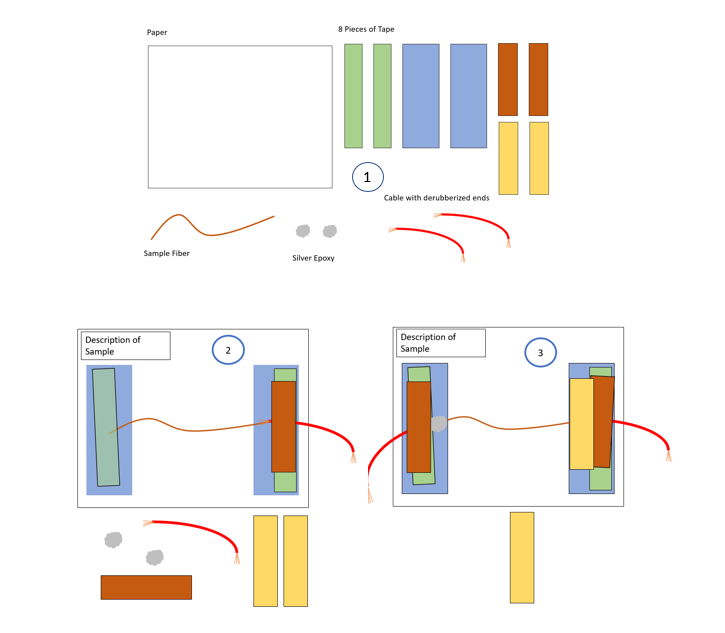
\includegraphics[width=\textwidth]{./pic/Meas_Prep_Together.PNG}
	\caption{Preparation for 
		Strain-Resistance-Measurement. \\
		Figure 2.4 shows cable with equivalent of brown tape.}
	\label{fig:MeasPrep}
\end{figure}


Prerequisites:

\begin{multicols}{2}
\begin{itemize}
    \item Sample with size $l$
    \item A small piece of paper
    \item 8 Pieces of Tape
    \item Silver Epoxy
    \item Derubberized Cable
\end{itemize}
\end{multicols}


Protocol:

\begin{enumerate}
	
    \item On piece of paper, put 1 piece of tape (Tape 1) on each side with distance $d < l$ from each other
    
    \item Now fix both ends of the sample gently without stretching (!) on Tape 1 with another piece of tape (Tape 2).
    
    \item Then, put free end of cable on end of sample, which is free and over Tape 1. Establish contact and fix cable with Tape 3.
    
    \item Put Silver Epoxy on sample-cable-interface to facilitate sample-cable-transmission. Bake at 80\textdegree C for 2h. After taking out the oven, put tape 4 perfectly aligned with the medial edge of Tape 1.
\end{enumerate}

    \begin{center}
    
See figure number \ref{fig:MeasPrep} for visual description of resistance measurement preparation.
    \end{center}


\subsubsection[Resistance Measurement]{Resistance Measurement \label{subsec:ResMeas} \footnote{For more extensive protocol, see page \pageref{App:ResMeas}}}

\begin{figure}[H]
    \centerline{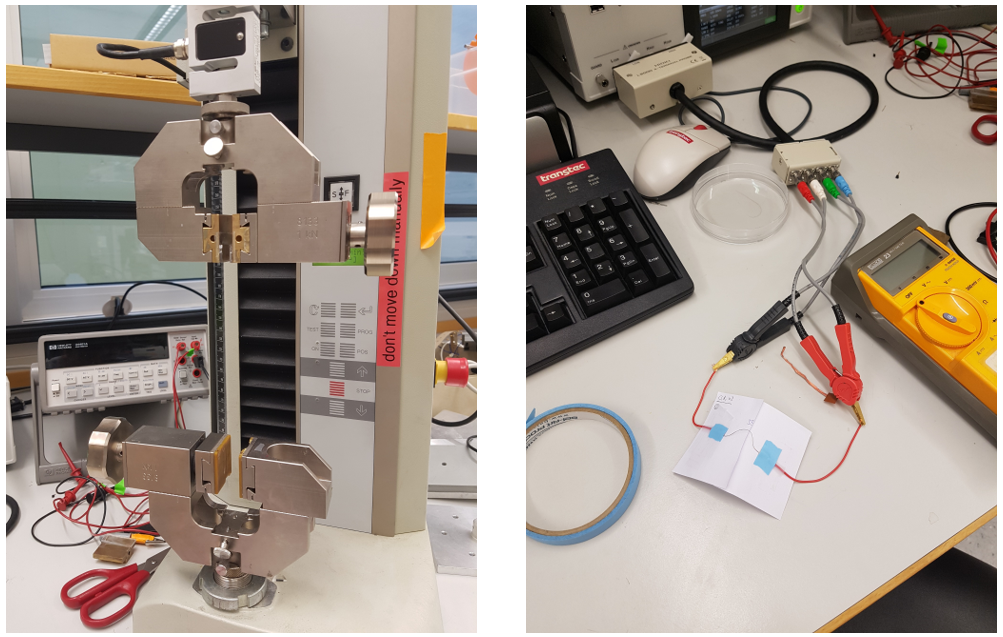
\includegraphics[scale=0.7]{./pic/MethodsResMeasurement.PNG}}
    \caption{Setup of Continuous Resistance Measurement}
    \label{fig:ContResMeas}
\end{figure}

Protocol:

\begin{enumerate}
	\item Cut the paper where sample is fixed on and tuck it in Zwick Roell Tensile Testing machine. 
	
	\item Increase the clamp-distance by 1\% of the initially measured sample length after every 30s that passed since start of measurement. 
	
	\item Stop measurement when either previously defined maximum strain is reached, conductivity is lost or measured conductivity is implausible.
	
	\item Process data by averaging datapoints that is included in the corresponding strain interval.

\end{enumerate}

